%------------------------------------------------------------------------------
\chapter{Methodology}
\label{ch:methodology}

Not only explain in more detail every equation, what it means, comparison with other papers and ideally improvements or were it fails at least.
Should I explain what is and how to do ray marching? What is the spectrum? How to integrate it to RGB coefficients?
Add all the values for the constants here or in implementation details??

Given simulated or captured fire data, that could come from any of the methods discussed in Section~\ref{sec:simulation}, we want to generate a photo-realistic image from a camera view of the scene.
From this point onwards we will assume that we have a volumetric data structure, which holds the relevant input data for the fire.

\section{Radiative Transport Equation}
\label{sec:radiative_transport_equation}

The Radiative Transport Equation (RTE) \cite{Howell:2002} models the variation of spectral radiance $(\omega \nabla) L(\lxo)$ in the medium, where $\lambda$ is a given wavelength in $m$, $\x$ is the point of interest in space, and $\omegam$ is a vector that points towards the viewing direction.
Formally, the objective is to get a solution for the RTE for each visible point in the scene, practically, an approximate solution will be computed.

\begin{figure}[htbp!]
	\centering
	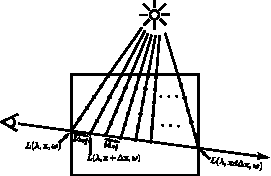
\includegraphics[width=0.8\textwidth]{img/ray_marching}
	\caption{Calculating the illumination values for samples along a ray.}
	\label{fig:ray_marching1}
\end{figure}

The integro-differential Radiative Transport Equation is defined as

\begin{equation}
\begin{split}
(\omega \nabla) L(\lxo) = &- \sigma_a(\lambda, \x) L(\lxo) + \sigma_a(\lambda, \x) L_e(\lxo) \\
&- \sigma_s(\lambda, \x) L(\lxo) + \sigma_s(\lambda, \x) L_i(\lxo),
\end{split}
\end{equation}

where $L_i$ is defined by

\begin{equation}
\label{eq:li}
L_i(\lxo) = \int_{4 \pi} L(\lxo_i) \Phi (\lambda, \omegam, \omegam_i) d \omegam_i,
\end{equation}

where $\sigma_a$ is an absorption coefficient, $\sigma_s$ is a scattering coefficient, $L_e$ is the emitted spectral radiance at the point, $L_i$ is the in-scattering radiance, $\Phi$ is a scattering phase function and $\omega_i$ is a scattering sampling direction.
In order to get an analytical solution to the aforementioned equation, the properties of the medium are assumed to be homogeneous over a small segment $\deltax$ in space,

\begin{equation}
\label{eq:rte_solution_paper}
\begin{split}
L(\lambda, \x + \Delta\x, \omegam) &= e^{-\sigma_t(\lambda, \x) \deltax} L(\lxo) +  \\
& (1 - e^{-\sigma_t(\lambda, \x) \deltax} ) \frac{\sigma_a(\lambda, \x) L_e(\lxo) + \sigma_s(\lambda, \x) L_i(\lxo)}{\sigma_t(\lambda, \x)},
\end{split}
\end{equation}

where $\sigma_t = \sigma_a + \sigma_s$ is the extinction coefficient, a visual depiction on this solution is shown in Figure~\ref{fig:ray_marching1}.
Examining each individual term in Equations~\ref{eq:li} and ~\ref{eq:rte_solution_paper}, the following factors will demand a more detailed definition

\begin{itemize}
\item Light \textbf{scattering} in the media, $\Phi(\lambda, \omegam, \omegam_i)$
\item Emitted light by \textbf{black body radiation}, $L_e(\lxo)$
\item Electromagnetic \textbf{absorption}, $\sigma_a$, of certain wavelengths 
\item Photons may follow non linear paths $\Delta\x$, due to spatially varying \textbf{refractive} indices
\item The eyes response to the final radiance $L(\lxo)$ is modified through \textbf{visual adaptation} processes
\end{itemize}

In the interest of simplicity, the absorption and radiation effects for \textbf{soot} will be treated separately from those caused by \textbf{other chemical species}.

\section{Scattering}
\label{sec:scattering}

The scattering phase function is defined by

\begin{equation}
\Phi (\lambda, \omegam, \omegam_i) = \frac{1 - g(\lambda)^2}{4 \pi(1 + g(\lambda)^2 - 2 g(\lambda) \omegam \omegam_i)^{\frac{3}{2}}},
\end{equation}

where $g$ can be a function of the wavelength, although in most cases is chosen to be constant.
The value of $g$ must be in the range $(-1, 1)$, where $g < 0$ corresponds to backwards scattering, $g = 0$ to isotropic scattering, and $g > 0$ to forwards scattering.

\section{Black Body Radiation}
\label{sec:black_body_radiation}

Emitted light $L_e(\lxo)$ from an idealized physical body that absorbs all incident electromagnetic radiation can be modelled with Planck's equation for black body radiation.
This equation characterizes the electromagnetic radiation $B(T, \lambda, \eta)$ emitted by a black body in thermal equilibrium at a given temperature $T$.

\begin{equation}
L_e(\lxo) = B(T, \lambda, \eta) = \frac{2 h c^2}{\lambda^5  (e ^\frac{h c}{\lambda k T} - 1)},
\end{equation}

where $h = 6.62606957 \times 10^{-34}~J/s$ is Planck's constant, $k = 1.3806488 \times 10^{-23}~J/K$ is Boltzmann constant and $c =  c_0 / \eta$ is the speed of light in the current medium, where $c_0 = 299792458~m/s$ is the speed of light in a vacuum and $\eta$ is the refraction index of the medium.
The refraction index $\eta$ varies across the medium, the procedure to compute will be described in Section~\ref{sec:refraction}.

\section{Absorption coefficients}
\label{sec:absorption_coefficients}

As fire is not an idealized black body radiator, certain wavelengths are not present in the emitted radiance.
This behaviour can be modelled using absorption coefficients for each chemical that would mask the undesired wavelengths, such that

\begin{equation}
\sigma_a L_e(\lxo) = \sum_{i = 0}^N \sigma_{ai} B_i(T, \lambda, \eta),
\end{equation}

where $N$ is the number of different chemical species in the mix, $\sigma_{ai}$ and $B_i(T, \lambda, \eta)$ are the absorption coefficient and light emission of the $i^{th}$ chemical.

\subsection{Soot Absorption}
\label{sec:soot_absorption}

The spectral absorption coefficient of soot is defined as

\begin{equation}
\sigma_a(\lambda, \x) = \frac{48 N(\x) \pi R^3 n m}{\lambda^{\alpha(\lambda)} ((n^2 - m^2 +2)^2 + 4 n^2 m^2)},
\end{equation}

where $N(\x)$ is the number density, density per unit volume, $R$ is the radius of a soot particle, $n$, $m$ and $\alpha(\lambda) = 1.39$ are optical constants for different types of soot.
In Table~\ref{tb:soot_absorption_coefficients}, values for the optical constants $n$ and $m$ are provided for several materials, the data was obtained from~\cite{Dalzell:1969}.
The radius of soot particles was determined in the range $R \in \lbrace 50\mbox{~\AA} \ldots 800\mbox{~\AA} \rbrace $ by~\cite{Dalzell:1969}.
Since our data is defined with soot densities, we have chosen the radius to be the mean value $R = 425 \times 10^{-10}$ metres.

\begin{table}[htbp!]
\centering
\caption{Absorption constants for propane and acetylene, wavelengths are in nanometres.}
\label{tb:soot_absorption_coefficients}
\begin{tabular}{cc|c|c|c|c|}
\cline{3-6}
                                                 &    & \multicolumn{4}{c|}{\textbf{Wavelengths}} \\ \cline{3-6} 
                                                 &    & 435.8   & 450    & 550   & 650   \\ \hhline{--|=|=|=|=|}
\multicolumn{1}{|c|}{\multirow{2}{*}{\textbf{Propane}}}   & \multicolumn{1}{c||}{n}  & 1.57    & 1.56   & 1.57  & 1.56  \\ \cline{2-6} 
\multicolumn{1}{|c|}{}                           & \multicolumn{1}{c||}{nm} & 0.46    & 0.5    & 0.53  & 0.52  \\ \hline
\multicolumn{1}{|c|}{\multirow{2}{*}{\textbf{Acetylene}}} & \multicolumn{1}{c||}{n}  & 1.56    & 1.56   & 1.56  & 1.57  \\ \cline{2-6} 
\multicolumn{1}{|c|}{}                           & \multicolumn{1}{c||}{nm} & 0.46    & 0.48   & 0.46  & 0.44  \\ \hline
\end{tabular}
\end{table}

\subsection{Absorption From Other Chemical Species}
\label{sec:absorption_from_chemical_species}

The emission and absorption coefficients associated with a given spectral frequency can be computed as


\begin{equation}
\sigma_a = \frac{\phi(\lambda) N_2 A_{21} \lambda^4 (e ^\frac{h c}{\lambda k T} - 1)}{8 \pi c}
\end{equation}

where $\phi(\lambda)$ is the normalized spectral line, $N_2$ is the number density of elements, $A_{21}$ is an Einstein coefficient measuring the transition probabilities of an spontaneous emission.

\section{Refraction}
\label{sec:refraction}

Assuming a negligible reflection index, the refraction angles for the rays can be easily computed using Snell's law

\begin{equation}
\frac{\sin \theta_1}{\sin \theta_2} = \frac{\eta_2}{\eta_1},
\end{equation}

where $\theta_1$ is the incident angle, $\theta_2$ is the refracted angle, $\eta_1$ is the index of refraction of the media which the ray is coming from and $\eta_2$ is the index of refraction of the media which the ray is going to.
The values for all the constants in this section are defined in Table~\ref{tb:ciddor_constants}.

\cite{Ciddor:1996} proposed a method to compute the refractive indices of air 

\begin{equation}
\label{eq:ciddor_eta_air}
\eta_{air} = 1 + \frac{\rho_a \eta_{axs}}{\rho_{axs}} + \frac{\rho_w \eta_{ws}}{\rho_{ws}},
\end{equation}

where $\rho_{axs}$ is the density of dry air, $\rho_{ws}$ is the density of pure water vapour, $\rho_{a}$ and $\rho_{w}$ are the equivalent quantities for dry air, $\eta_{axs}$ is the refractive index for $CO_2$ and $\eta_{ws}$ is the refractive index for water vapour.
The refractive index for $CO_2$ is estimated as

\begin{align}
\label{eq:ciddor_eta_axs}
\eta_{axs} &= \eta_{as} \left(1 + 0.534 \times 10^{-6} \left(x_c - 450 \right) \right), \\
\label{eq:ciddor_eta_as}
\eta_{as} &= 10^{-8} \left( \frac{k_1}{k_0 - \lambda} + \frac{k_3}{k_2 - \lambda} \right),
\end{align}

where $x_c \in \lbrace 300 \ldots 450 \rbrace $ is the proportion in ppm of $CO_2$, $k_0$, $k_1$ $k_2$ and $k_3$ are constants, and $\lambda$ is the wave number (reciprocal of the vacuum wavelength).
The refractive index for water vapour is computed as

\begin{equation}
\label{eq:ciddor_eta_ws}
\eta_{ws} = 1.022 \times 10^{-8} \left( w_0 + w_1 \lambda + w_1 \lambda^2 + w_3 \lambda^3 \right),
\end{equation}

where $w_0$, $w_1$, $w_2$ and $w_3$ are constants.

The $\rho$ densities are computed as follows

\begin{equation}
\label{eq:ciddor_rho}
\rho =  \frac{p m_a}{zrT} \left( 1 - x_w \left(1 - \frac{m_w}{m_a} \right) \right), 
\end{equation}

where $p$ is the pressure in pascals, $r$ and $m_w$ are constants, 

\begin{align}
\label{eq:ciddor_m_a}
m_a &= 0.0289635 + 12.011 \times 10^{-8}(x_c - 400)),\\
\label{eq:ciddor_z}
z &= 1 - \frac{p}{T} \left(a_0 + a_1 t + a_2 t^2 + \left(b_0 + b_1 t \right) x_w + \left(c_0 + c_1 t \right) x_w^2 \right) + \left( \frac{p}{T} \right)^2 \left( d + ex_w^2 \right),
\end{align}

where $a_0$,  $a_1$, $a_2$,  $b_0$,  $b_1$,  $c_0$,  $c_1$,  $d$ and $e$ are constants.

\begin{align}
\label{eq:ciddor_t}
T &= t + 273.15, \\
\label{eq:ciddor_x_w}
x_w &= \frac{f h v}{ p}, \\
\label{eq:ciddor_f}
f &= \alpha + \beta p + \gamma t^2,
\end{align}

where $\alpha$, $\beta$ and $\gamma$, and $h \in \lbrace 0 \ldots 1 \rbrace$ is the air relative fractional humidity, $0$ for dry air and given by the user for moist air.

The pressure $p$ can also be computed using the ideal gas law
\begin{equation}
\label{eq:ciddor_p}
pV=\frac{NRT}{V} = n T,
\end{equation}

where $N$ is the number of molecules, $V$ is the total volume of the gas, $T$ is the temperature of the gas, $n$ is the number density, $R = k N_a$, where $k$ is the Boltzmann constant and $N_a$ is Avogadro constant.

Depending on the situation, there are two acceptable methods to compute the vapour pressure $v$, both are described below.

\subsection{Davis' Saturation Vapour Pressure}
\label{subsec:davis_v}

In \cite{Ciddor:1996} paper, the author used the method proposed by~\cite{Davis:1992} to compute the saturation of vapour pressure

\begin{equation}
\label{eq:davis_v}
v = e^{AT^2 + BT + C + D/T},
\end{equation}

where $A$, $B$, $C$ and $D$ are constants.
This equation is relatively easy to compute, however incorrect results will be obtained for temperatures below $0\C$.
As we are concerned with fire rendering, which entails high temperatures, this method was chosen for its simplicity.

\subsection{Huang's Saturation Vapour Pressure}
\label{subsec:huang_v}

The International Association for the Properties of Water and Steam (IAPWS) adopted an alternative technique to~\cite{Davis:1992}, which was proposed by~\cite{Huang:1998}.
The more recent method will address the drawbacks of the previous one, giving reasonable results for temperatures below $0\C$, nevertheless, the generality comes with increased complexity in the equations.

\begin{align}
\label{eq:huang_v}
v &= 10^{6} \left( \frac{2C}{X} \right)^4, \\
X &= -B + \left( B^2 - 4AC \right)^{\frac{1}{2}}, \\
\begin{bmatrix}
A \\
B \\
C
\end{bmatrix} &=
\begin{bmatrix}
1 & K_1 & K_2 \\
K_3 & K_4 & K_5 \\
K_6 & K_7 & K_8 \\
\end{bmatrix} 
\begin{bmatrix}
~\Omega^2 \\
\Omega \\
1
\end{bmatrix}, \\
\Omega &= T + \frac{K_9}{T - K_{10}},
\end{align}

where $K_1$, $K_2$, $K_3$, $K_4$, $K_5$, $K_6$, $K_7$, $K_8$, $K_9$, and $K_{10}$ are constants.

\subsection{Ciddor's Method Summary}

The inputs of Ciddor's technique are a wavelength $\lambda_0$, a temperature $t$, a pressure $p$, a relative humidity value $h$ and a $CO_2$ concentration $x_c$.
The values for all the constants needed for the method are defined in Table~\ref{tb:ciddor_constants}.
The steps to compute the index of refraction are listed below

\begin{enumerate}
\item Precompute $z_a = 0.9995922115$, from Equation~\ref{eq:ciddor_z} with $t = 20~\C$, $p = 101.325~Pa$ and $x_w=0$.
\item Find $\lambda = 1 / \lambda_0^2$, and $T$ with Equation~\ref{eq:ciddor_t}.
\item Find $v$ with the method described in Section~\ref{subsec:davis_v} or in Section~\ref{subsec:huang_v}.
\item Find $x_w$ using Equations~\ref{eq:ciddor_f} and~\ref{eq:ciddor_x_w}.
\item Find $\eta_{as}$ using Equation~\ref{eq:ciddor_eta_as}.
\item Find $\eta_{ws}$ using Equation~\ref{eq:ciddor_eta_ws}.
\item Find $m_a$ using Equation~\ref{eq:ciddor_m_a}.
\item Find $\eta_{axs}$ using Equation~\ref{eq:ciddor_eta_axs}.
\item Find $z_m$ using Equation~\ref{eq:ciddor_z}.
\item Find $\rho_{axs} = (p_0 m_a)/(z_a r T_0)$, where $p_0 = 101325$, and $T_0 = 288.15$, using Equation~\ref{eq:ciddor_rho}.
\item Find $\rho_{w} = (x_w p m_w)/(z_m r T)$ using Equation~\ref{eq:ciddor_rho}.
\item Find $\rho_{a} = ((1 - x_w) p m_a)/(z_m r T)$ using Equation~\ref{eq:ciddor_rho}.
\item Find the index of refraction $\eta_{air}$ using Equation~\ref{eq:ciddor_eta_air}.
\end{enumerate} 

\begin{table}[]
\centering
\caption{Values for the constants in the equations used to compute the index of refraction.}
\label{tb:ciddor_constants}
\begin{tabular}{|l|l|l|l|l|}
\cline{1-2} \cline{4-5}
\textbf{Name}        & \textbf{Value}                       &  & \textbf{Name}     & \textbf{Value}                                \\ \cline{1-2} \cline{4-5} 
$\rho_{ws}$ & 0.00985938                  &  & $a_0$    & $1.58123~\times 10 ^{-6} K Pa^{-1}$  \\ \cline{1-2} \cline{4-5} 
$x_c$       & $450~ppm$                   &  & $a_1$    & $-2.9331 ~\times 10 ^{-8} Pa^{-1}$   \\ \cline{1-2} \cline{4-5} 
$k_0$       & $238.0185~\mu m^{-2}$       &  & $a_2$    & $1.1043 ~\times 10 ^{-10} Pa^{-1}$   \\ \cline{1-2} \cline{4-5} 
$k_1$       & $5792105~\mu m^{-2}$        &  & $b_0$    & $5.707~\times 10 ^{-6} K Pa^{-1}$    \\ \cline{1-2} \cline{4-5} 
$k_2$       & $57.362~\mu m^{-2}$         &  & $b_1$    & $-2.051~\times 10 ^{-8} Pa^{-1}$     \\ \cline{1-2} \cline{4-5} 
$k_3$       & $167917~\mu m^{-2}$         &  & $c_0$    & $1.9898~\times 10 ^{-4} K Pa^{-1}$   \\ \cline{1-2} \cline{4-5} 
$w_0$       & $295.235~\mu m^{-2}$        &  & $c_1$    & $-2.376~\times 10 ^{-6} K Pa^{-1}$   \\ \cline{1-2} \cline{4-5} 
$w_1$       & $2.6422~\mu m^{-2}$         &  & $d$      & $1.83~\times 10 ^{-11} K^2 Pa^{-2}$  \\ \cline{1-2} \cline{4-5} 
$w_2$       & $-0.03238~\mu m^{-2}$       &  & $e$      & $-0.765~\times 10 ^{-8} K^2 Pa^{-2}$ \\ \cline{1-2} \cline{4-5} 
$w_3$       & $0.004028~\mu m^{-2}$       &  & $\alpha$ & $1.00062$                            \\ \cline{1-2} \cline{4-5} 
$p$         & $1~atm~ = 101 325~Pa$       &  & $\beta$  & $3.14 \times 10^{-8} Pa^{-1}$        \\ \cline{1-2} \cline{4-5} 
$r$         & $8.31451~J mol^{-1} K^{-1}$ &  & $\gamma$ & $5.6 \times 10^{-7} \C^{-2}$         \\ \cline{1-2} \cline{4-5} 
$m_w$       & $0.018015~kg/mol$           &  & $k$      & $1.3806488 \times 10^{-23}~J/K$      \\ \cline{1-2} \cline{4-5} 
$N_a$ & $6.02214129 \times 10^{23}~mol^{-1}$ &  & $K_4$  & $1.20208247025 \times 10^{4}$   \\ \cline{1-2} \cline{4-5} 
$A$   & $1.2378847 \times 10^{-5} K^{-2}$    &  & $K_5$  & $-3.23255503223 \times 10^{6}$  \\ \cline{1-2} \cline{4-5} 
$B$   & $-1.9121316 \times 10^{-2} K^{-1}$   &  & $K_6$  & $1.49151086135 \times 10$       \\ \cline{1-2} \cline{4-5} 
$C$   & $33.93711047$                        &  & $K_7$  & $-4.82326573616 \times 10^{3}$  \\ \cline{1-2} \cline{4-5} 
$D$   & $-6.3431645 \times 10^3 K$           &  & $K_8$  & $4.05113405421 \times 10^{5}$   \\ \cline{1-2} \cline{4-5} 
$K_1$ & $1.16705214528 \times 10^{3}$        &  & $K_9$  & $-2.38555575678 \times 10^{-1}$ \\ \cline{1-2} \cline{4-5} 
$K_2$ & $-7.24213167032 \times 10^{5}$       &  & $K_{10}$ & $6.50175348448 \times 10^{2}$   \\ \cline{1-2} \cline{4-5} 
$K_3$ & $-1.70738469401 \times 10$           &  &        &                                 \\ \cline{1-2} \cline{4-5}
\end{tabular}
\end{table}

\section{Visual Adaptation}
\label{sec:visual_adaptation}

The human eye presents a non-linear response to incident radiance $L$, \cite{Naka:1966} proposed a simple equation to model this phenomena

\begin{equation}
\label{eq:visual_adaptation}
R(L, \tau) = \frac{L}{L + \tau},
\end{equation}

where $\tau$ is a non-linear adaptation state.
This state is determined by the visual system to maximize the perception of features for a given scene.

TALK SOMEWHERE ABOUT THE OTHER VISUAL ADAPTATION MODELS PRESENTED IN FAIRCHILD:2005
